\documentclass[12pt]{article}

\usepackage[a4paper, margin=2.5cm]{geometry}
\usepackage{graphicx}
\usepackage{rotating}
\usepackage[english]{babel}
\usepackage{appendix}
\usepackage{listings}
\usepackage{url}
\usepackage{todonotes}

\graphicspath{{./resources}}
  
\title{COMP3900-H15A-capSquad - Project Proposal}
\date{\today}
\author{Daniel Latimer z5115175 \\ Connor O'Shea z5115177 \\ Kevin Chan z5113136 \\ Oliver Richards z5157383 \\ Peter Kerr z5115807} 

\begin{document}

\maketitle
\tableofcontents
\newpage

\section{Background}

\begin{figure}
    
\includegraphics[width=\textwidth]{resources/spongebob}
    \caption{Background? \cite{Laird2012}}
    \label{fig:background}
\end{figure} \todo{delete me}

\subsection{Problem Domain}
\subsection{Existing Systems}

\section{User Stories}

\subsection{Product Backlog}

The 29 user stories which make up the product backlog, as shown in Figure XXX, were grouped into three categories as described in the sections 2.1.1-3.
Screenshots of the stories which make up the backlog can be found in sections 2.1.1-3.

\begin{figure}[h]
    \centering
    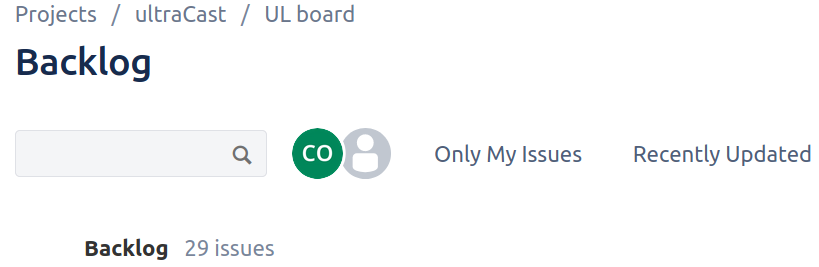
\includegraphics[width=10cm]{resources/project_backlog}
    \caption{ultraCast Backlog Count}
    \label{fig:background}
\end{figure}

\subsubsection{Project Objectives Stories}

The project objective stories were derived directly from the project objectives. These JIRA stories can be found in Figure XXX below.

\begin{figure}[h]
    \centering
    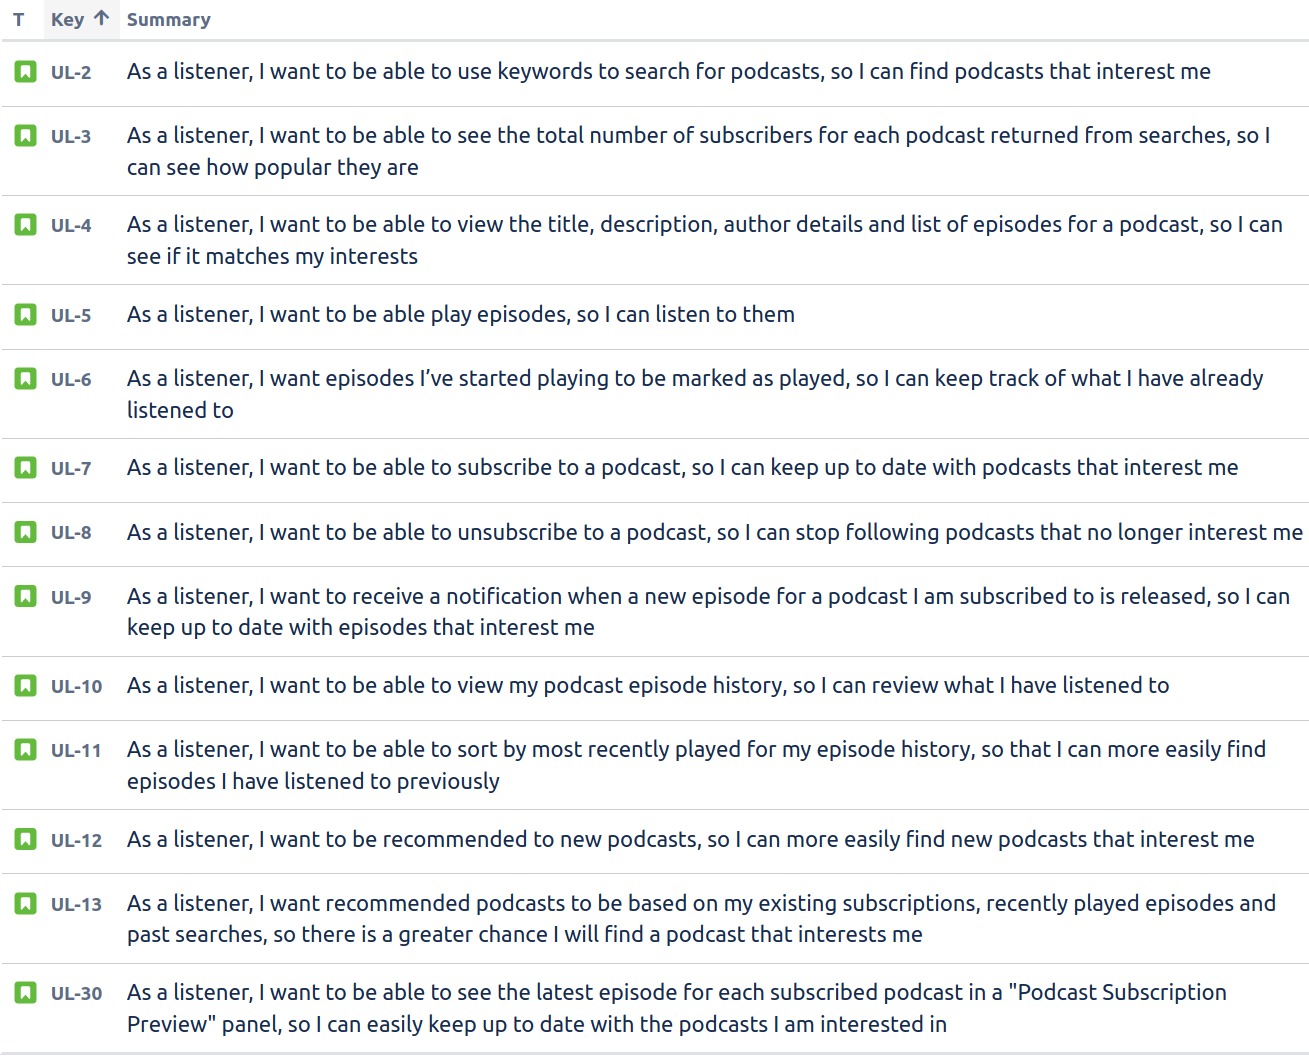
\includegraphics[width=\textwidth]{resources/objective_stories}
    \caption{JIRA Objective User Stories}
    \label{fig:background}
\end{figure}

The mapping of each project objective to the final user story was summarised in Table XXX.

\begin{table}[]
\caption{Project Objectives to Stories Mapping}
\begin{tabular}{|l|l|}
\hline
\textbf{Project Objective}                                                                                                                                                                                                                                                                                              & \textbf{\begin{tabular}[c]{@{}l@{}}Story\\ Key\end{tabular}} \\ \hline
\begin{tabular}[c]{@{}l@{}}Listeners must be able to search for podcasts that interest them by keywords, \\ resulting in a list of matching podcast titles, where the total number of \\ subscriptions on the ultraCast platform (function described later) for each \\ podcast is shown next to the title\end{tabular} & \begin{tabular}[c]{@{}l@{}}UL-2\\ UL-3\end{tabular}          \\ \hline
\begin{tabular}[c]{@{}l@{}}Listeners must be able to select a podcast show from returned search results\\ to view its full details, including its title, description, any author details that \\ exist, as well as a list of episodes for the show\end{tabular}                                                         & UL-4                                                         \\ \hline
\begin{tabular}[c]{@{}l@{}}Listeners must be able to play a selected episode within a podcast show, and \\ once that episode starts being played, the listener must be able to also clearly \\ see this episode marked as "Played"\end{tabular}                                                                         & \begin{tabular}[c]{@{}l@{}}UL-5\\ UL-6\end{tabular}          \\ \hline
Listeners must be able to subscribe or unsubscribe from a podcast show                                                                                                                                                                                                                                                  & \begin{tabular}[c]{@{}l@{}}UL-7\\ UL-8\end{tabular}          \\ \hline
\begin{tabular}[c]{@{}l@{}}Listeners must be able to see the latest episode available for each show that \\ they subscribed to in a "Podcast Subscription Preview" panel\end{tabular}                                                                                                                                   & UL-30                                                        \\ \hline
\begin{tabular}[c]{@{}l@{}}Listeners must be notified by the platform when a new episode for a show \\ they are subscribed appears\end{tabular}                                                                                                                                                                         & UL-9                                                         \\ \hline
\begin{tabular}[c]{@{}l@{}}Listeners must be able to see a history of the podcast episodes that they have\\ played, sorted in order from most recently played to least recently played\end{tabular}                                                                                                                     & \begin{tabular}[c]{@{}l@{}}UL-10\\ UL-11\end{tabular}        \\ \hline
\begin{tabular}[c]{@{}l@{}}ultraCast must be able to recommend new podcast shows to a listener based \\ on at least information about the podcast shows they are subscribed to, \\ podcast episodes they have recently played, and their past podcast searches\end{tabular}                                             & \begin{tabular}[c]{@{}l@{}}UL-12\\ UL-13\end{tabular}        \\ \hline
\end{tabular}
\end{table}


\subsubsection{System Stories}

The system stories were designed to address common features offered by existing offerings in the same problem domain. 
They can be seen in Figure XXX below.

\begin{figure}[h]
    \centering
    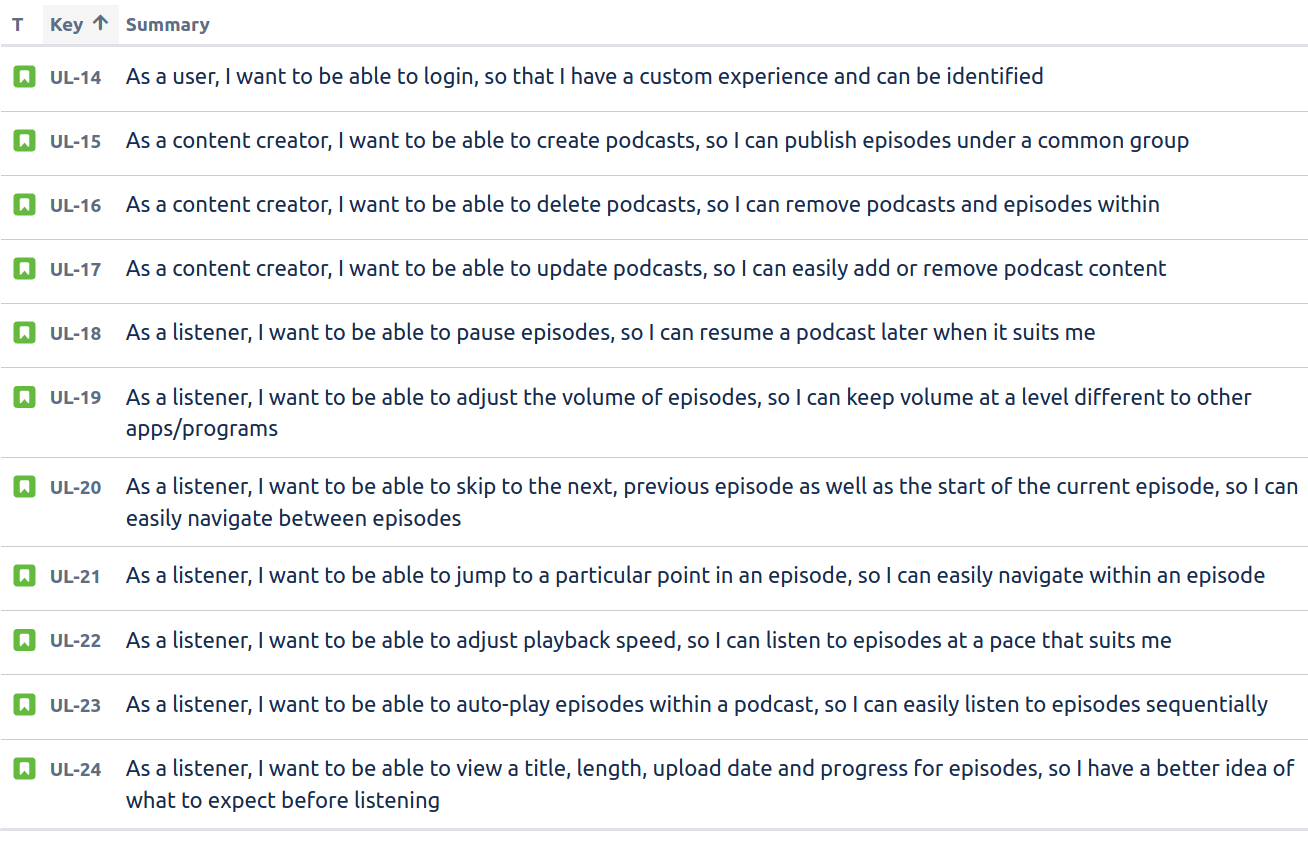
\includegraphics[width=\textwidth]{resources/system_stories}
    \caption{JIRA System User Stories}
    \label{fig:background}
\end{figure}

\subsubsection{Novel Features Stories}

The novel feature user stories, as shown in Figure XXX, were designed to create desirable features that are either uncommon or not 
available in other mainstream offerings in the same problem domain.

\begin{figure}[h]
    \centering
    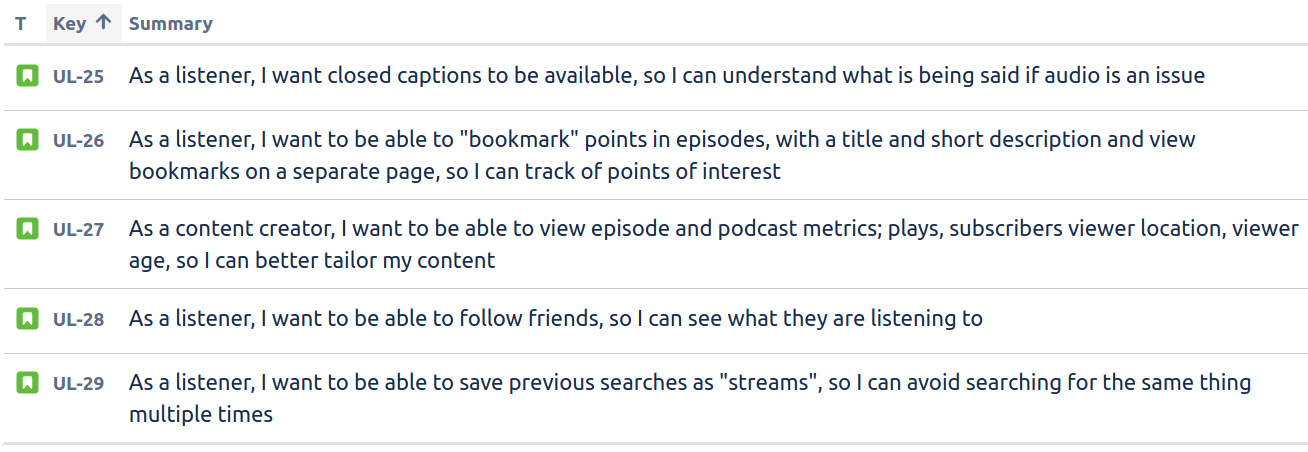
\includegraphics[width=\textwidth]{resources/novel_stories}
    \caption{JIRA Novel User Stories}
    \label{fig:background}
\end{figure}

TODO format as table using competitiors and user story numbers in figure above

\subsection{Sprints}
% Must have:
%   - Start + end dats of all sprints
%   - User stories in 1st sprint
%   - 

\section{Interface and Flow Diagrams}

\section{System Architecture}

The proposed system architecture can be seen in Figure \ref{fig:SysArch}.
First, we will use MongoDB to store our data, a NoSQL database that is popular for its high scalability.
This service will be interfaced with the MongoDB-Python driver, available on the MongoDB website.
Next, we will be using Flask for our web-server: a micro-framework that allows us to quickly develop an MVP solution.
Flask is written in Python, so connecting to the database via the MongoDB-Python driver should be straightforward.
Additionally, we will have a recommendation service that will generate recommended podcasts based on the users listening history.
Finally, we will have a React frontend application that will enable our users to login, search and play podcasts, and get recommendations on ones they may be interested in.
The React application and Flask application will communicate through a GraphQL API: a scalable alternative to the popular REST API.

The architecture has been designed with the final demonstration in mind, hence, the business and presentation layers are shown to be hosted on the VLab machine.
Currently, MongoDB is not supported by Debian 6 (the Linux environment on the VLab machine), so we have opted to put the data layer onto an AWS EC2 instance.

\begin{figure}[h]
    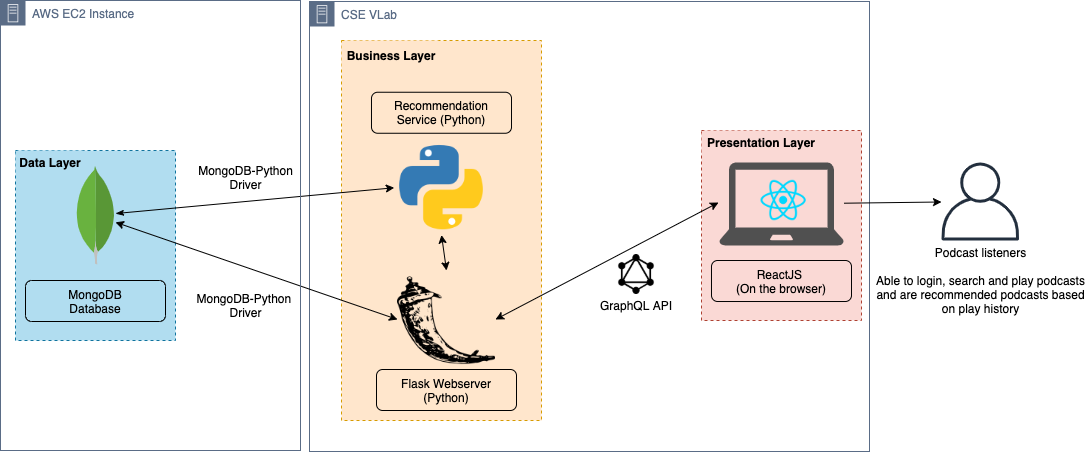
\includegraphics[width=\textwidth]{resources/SystemArchitecture}
    \caption{Proposed System Architecture}
    \label{fig:SysArch}
\end{figure}

\bibliography{library.bib}
\bibliographystyle{plain}
\end{document}
